\documentclass[a4paper]{article}

\usepackage[portuguese]{babel}
\usepackage{comment}
\usepackage[T1]{fontenc}
\usepackage[utf8]{inputenc}
\usepackage{hyperref}
\usepackage{graphicx}
\usepackage{float}
\usepackage{multirow}
\usepackage{indentfirst}
\usepackage[hypcap]{caption} % makes \ref point to top of figures and tables
\usepackage{lscape}

\graphicspath{ {images/} }

\begin{document}

\begin{titlepage}

	\begin{center}

		
\includegraphics[width=6cm]{./title}\\[3cm]

		\textsc{\LARGE Sistemas de Informação e Bases de Dados}\\[1.5cm]

		\textsc{\Large 1ª Parte do Projeto}\\[1.5cm]


		


		\noindent
		\begin{minipage}{0.4\textwidth}
			\begin{flushleft} \large
				Diogo Proença, 75313
			\end{flushleft}
		\end{minipage}
		\begin{minipage}{0.4\textwidth}
			\begin{flushright} \large
				Diogo Martins, 75462
			\end{flushright}
		\end{minipage}
		
		\begin{minipage}{0.4\textwidth}
			\begin{flushright} \large
				Bernardo Gomes, 75573	
			\end{flushright}
		\end{minipage}

		\vfill

		{\large \today}


	\end{center}

\end{titlepage}
\hypersetup{%
    pdfborder = {0 0 0}
}

\tableofcontents
\pagenumbering{gobble}
\pagebreak
\pagenumbering{arabic}
\section{Modelo E-R}
%explicações do modelo
\begin{landscape}
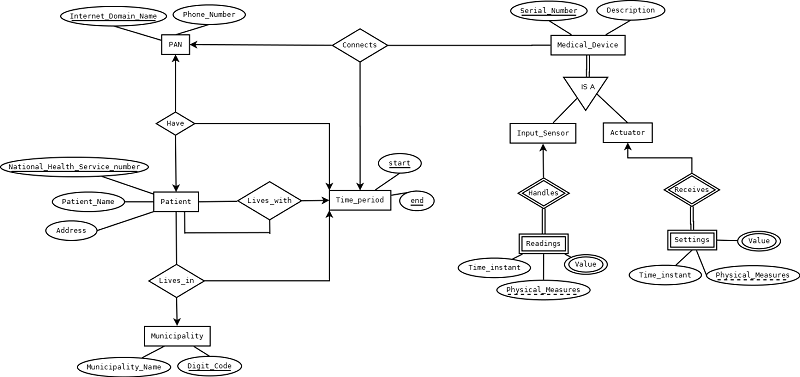
\includegraphics{Diagrama1.png}
\end{landscape}
\pagebreak

\section{Tabelas}


\end{document}